\section{Pytheas Algorithms}
\label{sec:pytheas:algo}


Using \idea, \name decouples real-time \mab into two parts:
a {\em session-grouping} logic to partition sessions into groups, and a {\em per-group \mab} logic
that makes per-session decisions. This section presents the design of these two core 
algorithmic pieces and how we address two issues:\footnote{We assume in this section that the per-group control logic is updated in real time (which will be made possible in the next section).} 
(i) Grouping drift: the session-grouping logic should dynamically regroup sessions based on the context that determines their QoE; 
and (ii) QoE drift: the per-group control logic should switch decisions when QoE of some decisions change. 



\subsection{Session-Grouping Logic}
\label{subsec:grouping}

Recall that sessions of the same group share the same factors on which their
QoE and best decisions depend.  As a concrete example, let us consider  CDN
selection for video.  Video sessions in the same AS whose QoE depends on the
local servers of different CDNs should be in the same group. However, video
sessions whose QoE is bottlenecked by home wireless and thus is independent to
CDNs should not be in the same group.  In other words, sessions in the
same group share not only the best decision, but also the factors that
determine the best decisions.

 A natural starting point for this grouping decision is 
 using the notion of critical features proposed in prior work~\cite{cfa}.  At a high level,
 if session A and B have the same values of  critical features,
 they will have similar QoE. 
% In the particular model, the space of decisions 
% (e.g., CDN, bitrate) is  simply another session feature.
Let  $\mathit{S}(s,F,\Delta)$ denote the 
  set of sessions that occur within the last $\Delta$ 
 time interval and share the same  feature values as $s$ on the set of features $F$, and 
 let $Q(X)$ denote the QoE distribution of a session set $X$. 
Then, the critical feature set $F^*$ of a session $s$:
%by the feature subset $F$ of $F^{all}$, such that 
\begin{displaymath}
\textrm{argmin}_{F\subseteq F^{\mathit{all}},  |S(s,F,\delta)| > n} | Q(S(s,F^{\mathit{all}},\Delta)) - Q(S(s,F,\Delta))| 
\end{displaymath}
% That is,  using  the 
% historical measurements matching just  $F^*$, we have a good  prediction of  the quality of the session $s$
% in the past over the $\Delta$ time interval (say last hour).
That is, the historical session who match values on critical features $F^*$ with $s$ 
have very similar QoE distribution to those matching on all features with $s$ on a 
long timescale of $\Delta$ (say last hour).
 The   clause $|S(s,F,\delta)| > n$  ensures that  there is sufficient mass in that set 
 to get a statistically significant estimate even on small timescales $\delta$ (e.g., minutes). 
%minimizes the difference between the QoE
%distributions of sessions which match on $F^{all}$ with $s$ in the last hour)
%and that of sessions $Q^{LastHour}(s,F)$ (which match on $F$ with $s$ in the last hour), and
% there are enough sessions matching on $F$.
 Such a notion of critical features has also been (implicitly) used in many other
applications; e.g., AS pairs in VoIP~\cite{via} and 
 /24 prefixes for web page load time~\cite{footprint}.
 Thus,  a natural strawman for grouping algorithm is to groups sessions who match on their critical features,
 i.e., they have similar QoE.
  

However, we observe two  problems inherent to critical features, which make
it unsuitable to directly group sessions based on critical features:
(1) First, grouping sessions based on critical features may result in groups that consist of
only sessions using similar decisions, so their measurement will be biased towards a subset of decisions.
(2) Second, grouping sessions based on critical features will also create overlaps between groups, so 
\mab logic of different groups could make conflicting decisions on these overlapping sessions.
%because when session $s_1$ matches its critical features with $s_2$, 
%$s_2$ may have a different set of critical features to $s_1$.
For instance, consider two Comcast sessions, $s_1$ and $s_2$, if the critical feature of $s_1$ is ISP, 
and the critical feature of $s_2$ is its local WiFi connection, 
$s_2$ will be in both the ``WiFi'' group and the ``Comcast'' group. 

%Realizing the similarity and fundamental difference between critical features and session grouping, 
To address these issues, we formulate the goal of session grouping as following.
Given a session set, the session-grouping logic should output any non-overlapping partition of sessions 
so that if two sessions $s_1$ and $s_2$ are in the same group, $s_1$ and $s_2$ should 
match values on $s_1$ or $s_2$'s non-decision-specific critical features. 
Non-decision-specific features are the features independent of decisions; e.g., ``device'' is a feature independent of decisions, since video sessions of the same device can make any decisions regarding CDN and bitrate.

Operationally, we use the following approach to achieve such a grouping.
First, for each session, we learn its critical features, and then ignore decision-specific features from the set of critical features of each session.
%Then, we group sessions so that 
%and then assigning overlapping parts to one of the overlapping groups.
%For instance, if B and C's groups overlap on A, we can simply assign A to B's group (or C's group), because the decision of A will not affect the logic of C's group, if A is in B's group.
%Note that this could lead to smaller groups than all sessions sharing values on their critical features, but as we will see in \Section\ref{sec:eval}\jc{Don't forget to result the results}, most sessions are in the groups with sufficient amount of sessions.
Then, we recursively group sessions based on the remaining critical features in a way that avoids overlaps between groups.
We start with any session $s_1$, and create a group consisting of all sessions that match with $s_1$ on $s_1$'s critical features.
We then recursively do the two following steps until every session is in some group.
We find a session $s_2$, who is not included in any existing group, and create a new group of all sessions that match with $s_2$ on $s_2$'s critical features.
If the new group does not overlap with any existing group, it will be a new individual group, otherwise, we will add it to the existing groups in the way illustrated in Figure~\ref{fig:grouping-example}.
%Figure~\ref{fig:grouping-example} shows how non-overlapping groups can be created by incrementally adding new groups based on critical features.
%At any point, 
We organize the existing groups in a graph, where each node is split by values of a certain feature, and each group includes multiple leaf nodes.
For instance, if we want to add a new group that consists of sessions whose ``content'' is ``Super Bowl'' to a graph of existing groups as shown in Figure~\ref{fig:grouping-example}a, we will fork a path to create a new leaf node whenever the new group overlap with a existing group.
Note that, this means multiple leaf nodes may be belong to the same group (e.g., ``Group 3'' in Figure~\ref{fig:grouping-example}b contains two different leaf nodes).

%The session-grouping logic also handles grouping drifts caused by sudden changes in workload, such as flashcrowd. We will be discuss it in \Section\ref{subsec:flashcrowd}.

%\camera{The session-grouping logic also will dynamically regroup sessions to handle frontend failure. We will discuss it in \Section\ref{subsec:fault}.}

%
%\vyas{here is the structure of this:
%
%1. Start with CFA formula of mathematical problem that CFA is solvng \\
%
%2. Then say here are two key reasons why it wont work -- a. it includes decision b. it can overlap \\
%
%3. Intuitively how to fix a/b \\
%
%4. What does group formula look like for the mathematical problem  \\
%}



%Note, however, \mab has different requirement than QoE prediction, which
%renders critical features not directly useful.  At first glance, we could group
%sessions who match on critical features, but this will create overlaps between
%groups, over which \mab logic of different groups could make conflicting
%decisions. Consider that session A matches on its critical feature with B and
%C, but session B and C do not match on their critical features. While this is
%allowed for QoE prediction, in \idea, the logic of B's group and that C's group
%might make different decisions for A. 


\begin{figure}[t!]
\centering
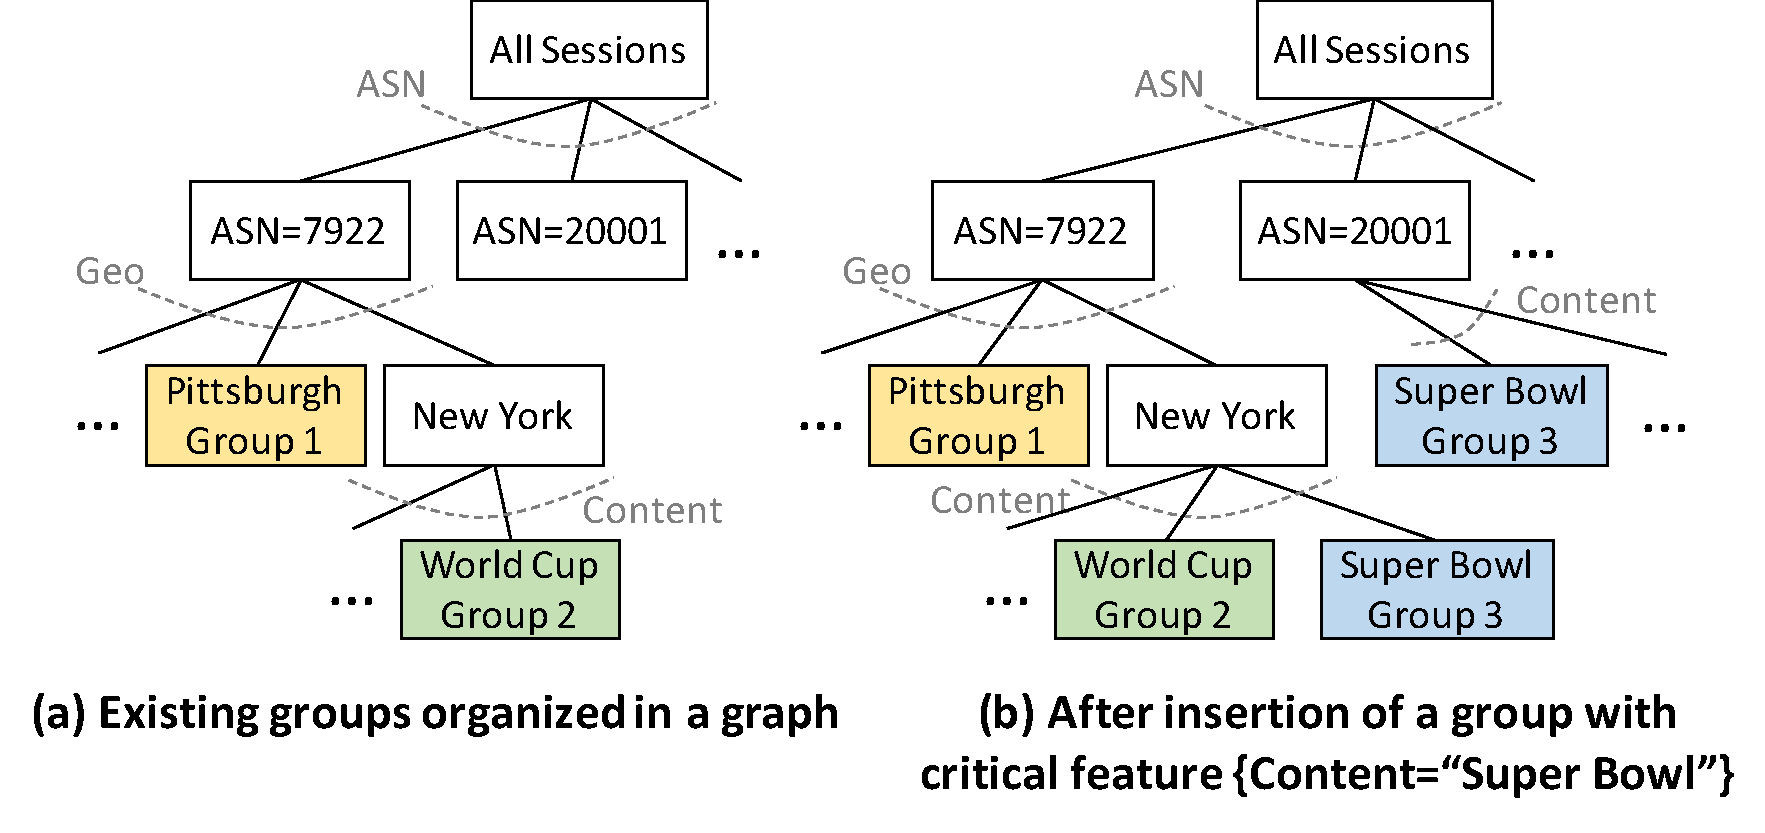
\includegraphics[width=0.85\textwidth]{figures/pytheas-grouping-example-2.pdf}
\caption{An illustrative example of session groups organized in a graph and how to a new group is added.}
\label{fig:grouping-example}
\end{figure}







\subsection{Per-Group \mab Logic}
\label{subsec:per-group}

To run \mab in presence of QoE drift, we use Discounted UCB
algorithm~\cite{discounteducb}, a variant of the UCB algorithm~\cite{ucb1}, as the
per-group \mab logic.  UCB (Upper Confidence Bound) algorithms~\cite{ucb1} are a
family of algorithms to solve the multi-armed bandits problem.  The core
idea is to always opportunistically choose the arm that has the highest
upper confidence bound of reward, and therefore, it will naturally tend to
use arms with high expected rewards or high
uncertainty. Note that the UCB algorithms do not explicitly assign sessions 
 for ``exploration'' and ``exploitation''.

We use Discounted UCB algorithm to adapt to QoE drift, because it automatically
gives more weight to more recent measurements by exponentially discounting
historical measurements.  Therefore, unlike other UCB algorithms which will
(almost) converge to one decision, Discounted UCB is more likely to revisit
suboptimal decisions to retain visibility across all decisions.
%As details of Discounted UCB can be found in~\cite{discounteducb}, we describe
%only its high level intuition here.  
We refer readers to~\cite{discounteducb} for more details.
Given a session $s$, it
returns a decision that has not been tried, if there is any.  Otherwise, it
calculates a score for each potential decision $\DecisionIndex$ by adding up an
exponentially weighted moving average of $\DecisionIndex$'s history QoE and an
estimation on the uncertainty of reward of $\DecisionIndex$, and picks
the decision with highest score.


%\vyas{is there any "adaptation" or extension of the algorithm to this context? if
% so try to highlight that} 


%$\bar{\QualityMean}(\gamma,\DecisionIndex)+{\QualityVariance}(\gamma,\DecisionIndex)$.
%Here, $\bar{\QualityMean}(\gamma,\DecisionIndex)$ is an exponentially weighted moving average of QoE of history sessions that used $\DecisionIndex$, 
%and ${\QualityVariance}(\gamma,\DecisionIndex)$ is an estimation on the uncertainty of reward of $\DecisionIndex$.
%By default, we use $\gamma=0.9$, which has good empirical performance.



